\documentclass{beamer}
\usepackage[utf8]{inputenc}
\usepackage{graphicx, epsfig}
\usepackage{amsmath,mathrsfs,amsfonts,amssymb}
\usepackage{floatflt}
\usepackage{epic,ecltree}
\usepackage{mathtext}
\usepackage{fancybox}
\usepackage{fancyhdr}
\usepackage{multirow}
\usepackage{enumerate}
\usepackage{epstopdf}
\usepackage{multicol}
\usepackage{algorithm}
\usepackage[noend]{algorithmic}
\usepackage{tikz}
\usepackage{blindtext}
\usetheme{default}%{Singapore}%{Warsaw}%{Warsaw}%{Darmstadt}
\usecolortheme{default}

\setbeamerfont{title}{size=\Huge}
\setbeamertemplate{footline}[page number]{}

\setbeamertemplate{section in toc}[sections numbered]


\makeatletter
\newcommand\HUGE{\@setfontsize\Huge{35}{40}}
\makeatother    

\setbeamerfont{title}{size=\HUGE}
\beamertemplatenavigationsymbolsempty

% latin bold lower
\newcommand{\ba}{\mathbf{a}} 
\newcommand{\bc}{\mathbf{c}} 
\newcommand{\be}{\mathbf{e}} 
\newcommand{\bh}{\mathbf{h}} 
\newcommand{\bp}{\mathbf{p}} 
\newcommand{\bt}{\mathbf{t}} 
\newcommand{\bs}{\mathbf{s}} 
\newcommand{\bu}{\mathbf{u}} 
\newcommand{\bv}{\mathbf{v}} 
\newcommand{\bw}{\mathbf{w}} 
\newcommand{\bx}{\mathbf{x}} 
\newcommand{\by}{\mathbf{y}} 
\newcommand{\bz}{\mathbf{z}} 

% latin bold upper
\newcommand{\bA}{\mathbf{A}} 
\newcommand{\bB}{\mathbf{B}} 
\newcommand{\bC}{\mathbf{C}} 
\newcommand{\bI}{\mathbf{I}} 
\newcommand{\bL}{\mathbf{L}} 
\newcommand{\bM}{\mathbf{M}} 
\newcommand{\bQ}{\mathbf{Q}} 
\newcommand{\bT}{\mathbf{T}} 
\newcommand{\bU}{\mathbf{U}} 
\newcommand{\bV}{\mathbf{V}} 
\newcommand{\bW}{\mathbf{W}} 
\newcommand{\bX}{\mathbf{X}} 
\newcommand{\bY}{\mathbf{Y}} 
\newcommand{\bZ}{\mathbf{Z}} 

% latin cal upper
\newcommand{\cG}{\mathcal{G}} 
\newcommand{\cL}{\mathcal{L}} 
\newcommand{\cN}{\mathcal{N}} 
\newcommand{\cS}{\mathcal{S}} 
\newcommand{\cT}{\mathcal{T}} 
\newcommand{\cW}{\mathcal{W}} 
\newcommand{\cX}{\mathcal{X}} 
\newcommand{\cZ}{\mathcal{Z}} 

% latin bb upper
\newcommand{\bbE}{\mathbb{E}} 
\newcommand{\bbI}{\mathbb{I}} 
\newcommand{\bbP}{\mathbb{P}} 
\newcommand{\bbR}{\mathbb{R}} 

% greek bold lower
\newcommand{\bepsilon}{\boldsymbol{\epsilon}} 
\newcommand{\btheta}{\boldsymbol{\theta}} 
\newcommand{\blambda}{\boldsymbol{\lambda}} 
\newcommand{\bpi}{\boldsymbol{\pi}} 
\newcommand{\bmu}{\boldsymbol{\mu}} 
\newcommand{\bsigma}{\boldsymbol{\sigma}} 
\newcommand{\bphi}{\boldsymbol{\phi}} 

% greek bold upper
\newcommand{\bSigma}{\boldsymbol{\Sigma}} 

\DeclareMathOperator*{\argmin}{arg\,min}
\DeclareMathOperator*{\argmax}{arg\,max}

\newcommand{\createdgmtitle}[1]{\title[\hbox to 56mm{Deep Generative Models  \hfill\insertframenumber\,/\,\inserttotalframenumber}]
	{Deep Generative Models \\ {\Huge Lecture #1}}
	\author{Roman Isachenko}
	\institute{
\includegraphics[width=0.5cm]{../utils/ozonmasterslogo} \large{Ozon Masters}}
	\date{Spring, 2022}
}

\newcommand\myfootnote[1]{%
  \tikz[remember picture,overlay]
  \draw (current page.south west) +(1in + \oddsidemargin,0.5em)
  node[anchor=south west,inner sep=0pt]{\parbox{\textwidth}{%
      \rlap{\rule{10em}{0.4pt}}\raggedright\scriptsize \textit{#1}}};}

\newcommand\myfootnotewithlink[2]{%
  \tikz[remember picture,overlay]
  \draw (current page.south west) +(1in + \oddsidemargin,0.5em)
  node[anchor=south west,inner sep=0pt]{\parbox{\textwidth}{%
      \rlap{\rule{10em}{0.4pt}}\raggedright\scriptsize\href{#1}{\textit{#2}}}};}
      
\AtBeginSection[]
{
	\begin{frame}{Outline}
		\tableofcontents[currentsection,subsectionstyle=hide]
	\end{frame}
}
\AtBeginSubsection[]{
	\begin{frame}{Outline}
		\tableofcontents[currentsection,currentsubsection]
	\end{frame}
}
\createdgmtitle{13}

\usepackage{tikz}

\usetikzlibrary{arrows,shapes,positioning,shadows,trees}
%--------------------------------------------------------------------------------
\begin{document}
%--------------------------------------------------------------------------------
\begin{frame}[noframenumbering,plain]
%\thispagestyle{empty}
\titlepage
\end{frame}
%=======
\begin{frame}{Outline}
	\tableofcontents
\end{frame}
%=======
\begin{frame}{Recap of previous lecture}
	\begin{block}{Discrete VAE latents}
		\begin{itemize}
			\item Define dictionary (word book) space $\{\be_k\}_{k=1}^K$, where $\be_k \in \bbR^C$, $K$ is the size of the dictionary.
			\item Our variational posterior $q(c | \bx, \bphi) = \text{Categorical}(\bpi(\bx, \bphi))$ (encoder) outputs discrete probabilities vector.
			\item We sample $c^*$ from $q(c | \bx, \bphi)$ (reparametrization trick analogue).
			\item Our generative distribution $p(\bx | \be_{c^*}, \btheta)$ (decoder).
		\end{itemize}
	\end{block}
	\begin{block}{ELBO}
		\vspace{-0.5cm}
		\[
			\mathcal{L} (\bphi, \btheta)  = \mathbb{E}_{q(c | \bx, \bphi)} \log p(\bx | c, \btheta) - KL(q(c| \bx, \bphi) || p(c)) \rightarrow \max_{\bphi, \btheta}.
		\]
		\vspace{-0.5cm}
	\end{block}
	\begin{block}{KL term}
		\vspace{-0.4cm}
		\[
			KL(q(c| \bx, \bphi) || p(c)) = - H(q(c | \bx, \bphi)) + \log K. 
		\]
	\end{block}
\end{frame}
%=======
\begin{frame}{Recap of previous lecture}
	\begin{figure}
		\centering
		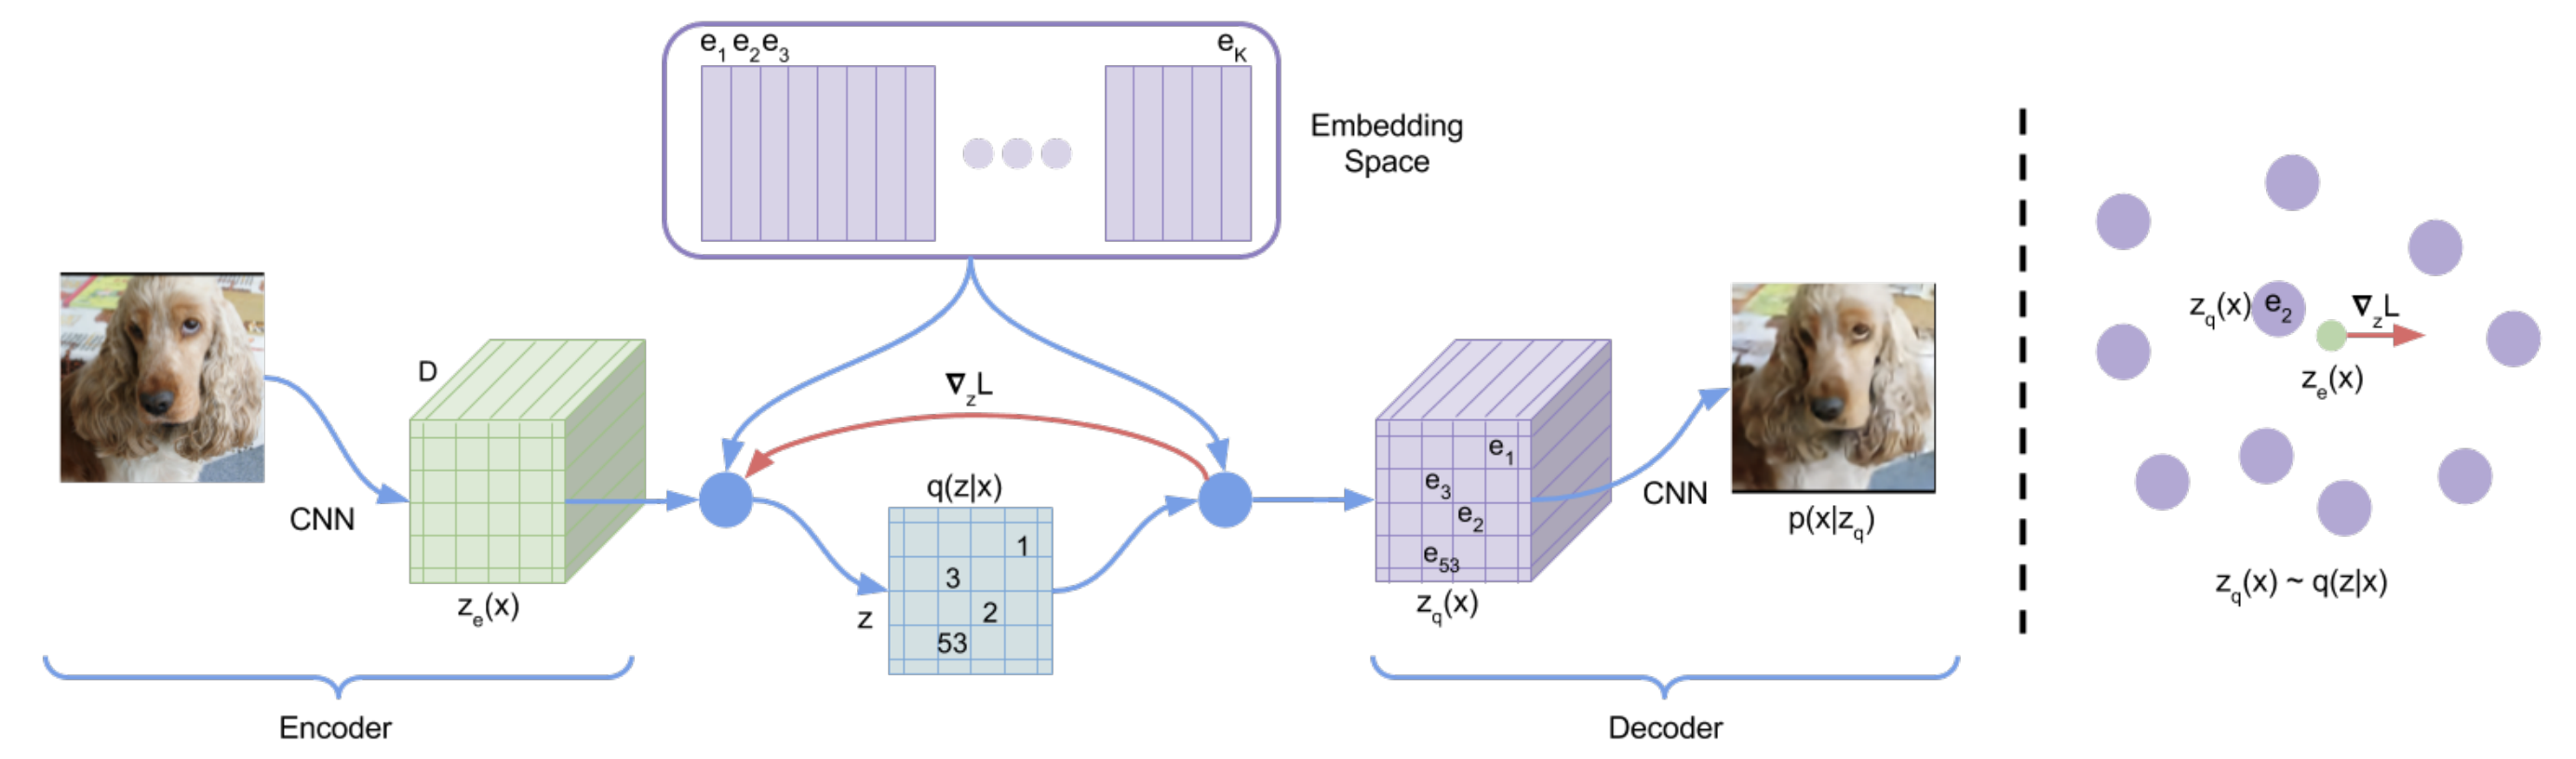
\includegraphics[width=0.85\linewidth]{figs/vqvae}
	\end{figure}
	\vspace{-0.3cm}
	\begin{block}{Deterministic variational posterior}
		\vspace{-0.8cm}
		\[
			q(c_{ij} = k^* | \bx, \bphi) = \begin{cases}
				1 , \quad \text{for } k^* = \argmin_k \| [\bz_e]_{ij} - \be_k \|; \\
				0, \quad \text{otherwise}.
			\end{cases}
		\]
		\vspace{-0.8cm}
	\end{block}
	\begin{block}{ELBO}
		\vspace{-0.6cm}
		\[
			\mathcal{L} (\bphi, \btheta)  = \mathbb{E}_{q(c | \bx, \bphi)} \log p(\bx | \be_{c} , \btheta) - \log K =  \log p(\bx | \bz_q, \btheta) - \log K.
		\]
		\vspace{-0.6cm}
	\end{block}
	\begin{block}{Straight-through gradient estimation}
		\vspace{-0.6cm}
		\[
			\frac{\partial \log p(\bx | \bz_q , \btheta)}{\partial \bphi} = \frac{\partial \log p(\bx | \bz_q, \btheta)}{\partial \bz_q} \cdot {\color{red}\frac{\partial \bz_q}{\partial \bphi}} \approx \frac{\partial \log p(\bx | \bz_q, \btheta)}{\partial \bz_q} \cdot \frac{\partial \bz_e}{\partial \bphi}
		\]
	\end{block}
	\myfootnotewithlink{https://arxiv.org/abs/1711.00937}{Oord A., Vinyals O., Kavukcuoglu K. Neural Discrete Representation Learning, 2017} 
\end{frame}
%=======
\begin{frame}{Recap of previous lecture}
	\vspace{-0.4cm}
	\begin{block}{Gumbel-max trick}
		Let $g_k \sim \text{Gumbel}(0, 1)$ for $k = 1, \dots, K$. Then
		\vspace{-0.3cm}
		\[
			c = \argmax_k [\log \pi_k + g_k]
		\]
		\vspace{-0.6cm} \\
		has a categorical distribution $c \sim \text{Categorical}(\bpi)$.
	\end{block}
	\vspace{-0.2cm}
	\begin{block}{Gumbel-softmax relaxation}
		Concrete distribution = continuous + discrete
		\vspace{-0.2cm}
		\[
			\hat{c}_k = \frac{\exp \left(\frac{\log q(k | \bx, \bphi) + g_k}{\tau}\right)}{\sum_{j=1}^K \exp \left(\frac{\log q(j | \bx, \bphi) + g_j}{\tau}\right)}, \quad k = 1, \dots, K.
		\]
		\vspace{-0.7cm}
 	\end{block}
	\begin{block}{Reparametrization trick}
		\vspace{-0.4cm}
		\[
			\nabla_{\bphi} \mathbb{E}_{q(c | \bx, \bphi)} \log p(\bx | \be_{c} , \btheta) = \bbE_{\text{Gumbel}(0, 1)} \nabla_{\bphi} \log p(\bx | \bz , \btheta),
		\]
		where $\bz = \sum_{k=1}^K\hat{c}_k \be_k$ (all operations are differentiable now).
	\end{block}
 	\vspace{-0.2cm}
	\myfootnote{
	\href{https://arxiv.org/abs/1611.00712}{Maddison C. J., Mnih A., Teh Y. W. The Concrete distribution: A continuous relaxation of discrete random variables, 2016} \\
	\href{https://arxiv.org/abs/1611.01144}{Jang E., Gu S., Poole B. Categorical reparameterization with Gumbel-Softmax, 2016}
	}
\end{frame}
%=======
\begin{frame}{Recap of previous lecture}
	Consider Ordinary Differential Equation    
	\begin{align*}
	    \frac{d \bz(t)}{dt} &= f(\bz(t), \btheta); \quad \text{with initial condition }\bz(t_0) = \bz_0. \\
	    \bz(t_1) &= \int^{t_1}_{t_0} f(\bz(t), \btheta) d t  + \bz_0 = \text{ODESolve}(\bz(t_0), f, t_0,t_1, \btheta).
	\end{align*}
	\vspace{-0.4cm}
	\begin{block}{Euler update step}
		\vspace{-0.6cm}
		\[
		    \frac{\bz(t + \Delta t) - \bz(t)}{\Delta t} = f(\bz(t), \btheta) \quad \Rightarrow \quad \bz(t + \Delta t) = \bz(t) + \Delta t \cdot f(\bz(t), \btheta).
		\]
		\vspace{-0.7cm}
	\end{block}
	\begin{block}{Residual block}
		\vspace{-0.4cm}
		\[
			\bz_{t + 1} = \bz_t + f(\bz_t, \btheta)
		\]
		It is equavalent to Euler update step for solving ODE with $\Delta t = 1$!
	\end{block}
	In the limit of adding more layers and taking smaller steps we get: 
	\[
	    \frac{d \bz(t)}{dt} = f(\bz(t), t, \btheta); \quad \bz(t_0) = \bx; \quad \bz(t_1) = \by.
	\]

	\myfootnotewithlink{https://arxiv.org/abs/1806.07366}{Chen R. T. Q. et al. Neural Ordinary Differential Equations, 2018}   
\end{frame}
%=======

\begin{frame}{Neural ODE}
	\begin{block}{Forward pass (loss function)}
		\vspace{-0.8cm}
		\begin{align*}
			L(\by) = L(\bz(t_1)) &= L\left( \bz(t_0) + \int_{t_0}^{t_1} f(\bz(t), \btheta) dt \right) \\ &= L\bigl(\text{ODESolve}(\bz(t_0), f, t_0,t_1, \btheta) \bigr)
		\end{align*}
	\vspace{-0.5cm}
	\end{block}
	\textbf{Note:} ODESolve could be any method (Euler step, Runge-Kutta methods).
	\begin{block}{Backward pass (gradients computation)}
		For fitting parameters we need gradients:
		\[
			\ba_{\bz}(t) = \frac{\partial L(\by)}{\partial \bz(t)}; \quad \ba_{\btheta}(t) = \frac{\partial L(\by)}{\partial \btheta(t)}.
		\]
		In theory of optimal control these functions called \textbf{adjoint} functions. 
		They show how the gradient of the loss depends on the hidden state~$\bz(t)$ and parameters $\btheta$.
	\end{block}

	\myfootnotewithlink{https://arxiv.org/abs/1806.07366}{Chen R. T. Q. et al. Neural Ordinary Differential Equations, 2018}     
\end{frame}
%=======
\section{Neural ODE: finish}
%=======
\begin{frame}{Neural ODE}
	\begin{block}{Adjoint functions}
		\vspace{-0.3cm}
		\[
			\ba_{\bz}(t) = \frac{\partial L(\by)}{\partial \bz(t)}; \quad \ba_{\btheta}(t) = \frac{\partial L(\by)}{\partial \btheta(t)}.
		\]
		\vspace{-0.6cm}
	\end{block}
	\begin{block}{Theorem (Pontryagin)}
	\vspace{-0.6cm}
	\[
	     \frac{d \ba_{\bz}(t)}{dt} = - \ba_{\bz}(t)^T \cdot \frac{\partial f(\bz(t), \btheta)}{\partial \bz}; \quad \frac{d \ba_{\btheta}(t)}{dt} = - \ba_{\bz}(t)^T \cdot \frac{\partial f(\bz(t), \btheta)}{\partial \btheta}.
	\]
	Do we know any initilal condition?
	\end{block}
	\begin{block}{Solution for adjoint function}
		\vspace{-0.8cm}
		\begin{align*}
			 \frac{\partial L}{\partial \btheta(t_0)} &= \ba_{\btheta}(t_0) =  - \int_{t_1}^{t_0} \ba_{\bz}(t)^T \frac{\partial f(\bz(t), \btheta)}{\partial \btheta(t)} dt + 0\\
			 \frac{\partial L}{\partial \bz(t_0)} &= \ba_{\bz}(t_0) =  - \int_{t_1}^{t_0} \ba_{\bz}(t)^T \frac{\partial f(\bz(t), \btheta)}{\partial \bz(t)} dt + \frac{\partial L}{\partial \bz(t_1)}\\
		\end{align*}
		\vspace{-1.5cm}
	\end{block}
	\textbf{Note:} These equations are solved back in time.
	\myfootnotewithlink{https://arxiv.org/abs/1806.07366}{Chen R. T. Q. et al. Neural Ordinary Differential Equations, 2018}   
\end{frame}
%=======
\begin{frame}{Neural ODE}
	\vspace{-0.2cm}
	\begin{block}{Forward pass}
		\vspace{-0.5cm}
		\[
			\bz(t_1) = \int^{t_1}_{t_0} f(\bz(t), \btheta) d t  + \bz_0 \quad \Rightarrow \quad \text{ODE Solver}
		\]
		\vspace{-0.6cm}
	\end{block}
	\begin{block}{Backward pass}
		\vspace{-0.8cm}
		\begin{equation*}
			\left.
				{\footnotesize 
				\begin{aligned}
					\frac{\partial L}{\partial \btheta(t_0)} &= \ba_{\btheta}(t_0) =  - \int_{t_1}^{t_0} \ba_{\bz}(t)^T \frac{\partial f(\bz(t), \btheta)}{\partial \btheta(t)} dt + 0 \\
					\frac{\partial L}{\partial \bz(t_0)} &= \ba_{\bz}(t_0) =  - \int_{t_1}^{t_0} \ba_{\bz}(t)^T \frac{\partial f(\bz(t), \btheta)}{\partial \bz(t)} dt + \frac{\partial L}{\partial \bz(t_1)} \\
					\bz(t_0) &= - \int^{t_0}_{t_1} f(\bz(t), \btheta) d t  + \bz_1.
				\end{aligned}
				}
			\right\rbrace
			 \Rightarrow
			\text{ODE Solver}
		\end{equation*}
		\vspace{-0.4cm} 
	\end{block}
	\textbf{Note:} These scary formulas are the standard backprop in the discrete case.
	\begin{figure}
		\centering
		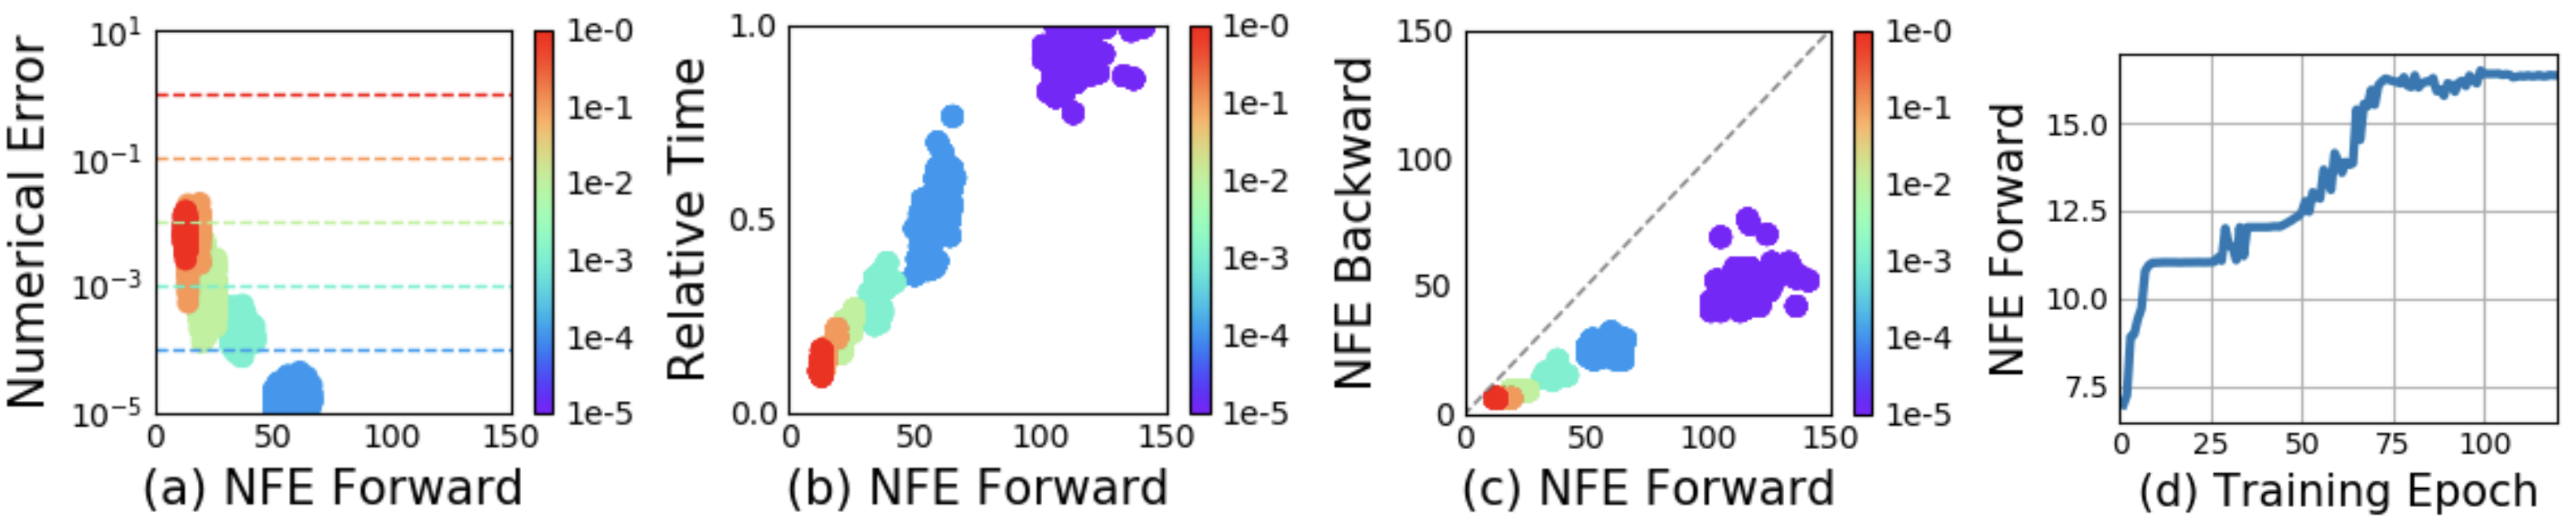
\includegraphics[width=\linewidth]{figs/neural_ode}
	\end{figure}
	\myfootnotewithlink{https://arxiv.org/abs/1806.07366}{Chen R. T. Q. et al. Neural Ordinary Differential Equations, 2018}   
\end{frame}
%=======
\section{Continuous-in-time normalizing flows}
%=======
\begin{frame}{Continuous Normalizing Flows}
	\begin{block}{Discrete Normalizing Flows}
		\vspace{-0.8cm}
		  \[
		  \bz_{t+1} = f(\bz_t, \btheta); \quad \log p(\bz_{t+1}) = \log p(\bz_{t}) - \log \left| \det \frac{\partial f(\bz_t, \btheta)}{\partial \bz_{t}} \right| .
		  \]
		\vspace{-0.7cm}
	\end{block}
	\begin{block}{Continuous-in-time dynamics}
		\vspace{-0.2cm}
		\[
			\frac{d\bz(t)}{dt} = f(\bz(t), \btheta).
		\]
		\vspace{-0.4cm}
	\end{block}
	Assume that function $f$ is uniformly Lipschitz continuous in $\bz$ and continuous in $t$. From Picard’s existence theorem, it follows that the above ODE has a \textbf{unique solution}.
	\begin{block}{Forward and inverse transforms}
		\vspace{-0.7cm}
		\begin{align*}
			\bx &= \bz(t_1) = \bz(t_0) + \int_{t_0}^{t_1} f(\bz(t), \btheta) dt \\
			\bz &= \bz(t_0) = \bz(t_1) + \int_{t_1}^{t_0} f(\bz(t), \btheta) dt \\
		\end{align*}
	\end{block}
	\myfootnotewithlink{https://arxiv.org/abs/1912.02762}{Papamakarios G. et al. Normalizing flows for probabilistic modeling and inference, 2019}   
\end{frame}
%=======
\begin{frame}{Continuous Normalizing Flows}
	To train this flow we have to get the way to calculate the density~$p(\bz(t), t)$.
	\begin{block}{Theorem (special case of Kolmogorov-Fokker-Planck)}
		if function $f$ is uniformly Lipschitz continuous in $\bz$ and continuous in $t$, then
		\[
			\frac{d \log p(\bz(t), t)}{d t} = - \text{tr} \left( \frac{\partial f (\bz(t), \btheta)}{\partial \bz(t)} \right).
		\]
		\vspace{-0.5cm}
	\end{block}
	\textbf{Note:} Unlike discrete-in-time flows, the function $f$ does not need to be bijective, because uniqueness guarantees that the entire transformation is automatically bijective.
	\begin{block}{Density evaluation}
		\vspace{-0.4cm}
		\[
			\log p(\bx | \btheta) = \log p(\bz) - \int_{t_0}^{t_1} \text{tr}  \left( \frac{\partial f (\bz(t), \btheta)}{\partial \bz(t)} \right) dt.
		\]
		Here $p(\bx | \btheta) = p(\bz(t_1), t_1)$, $p(\bz) = p(\bz(t_0), t_0)$. \\
		\textbf{Adjoint} method is used for getting the derivatives.
	\end{block}
	\myfootnotewithlink{https://arxiv.org/abs/1806.07366}{Chen R. T. Q. et al. Neural Ordinary Differential Equations, 2018}   
\end{frame}
%=======
\begin{frame}{Continuous Normalizing Flows}
	\vspace{-0.5cm}
	\begin{block}{Forward transform + log-density}
		\vspace{-0.5cm}
		\[
			\begin{bmatrix}
				\bx \\
				\log p(\bx | \btheta)
			\end{bmatrix}
			= 
			\begin{bmatrix}
				\bz \\
				\log p(\bz)
			\end{bmatrix} + 
			\int_{t_0}^{t_1} 
			\begin{bmatrix}
				f(\bz(t), \btheta) \\
				- \text{tr} \left( \frac{\partial f(\bz(t), \btheta)}{\partial \bz(t)} \right) 
			\end{bmatrix} dt.
		\]
		\vspace{-0.4cm}
	\end{block}
	\begin{itemize}
		\item Discrete-in-time normalizing flows need invertible $f$. It costs $O(m^3)$ to get determinant of the Jacobian.
		\item Continuous-in-time flows require only smoothness of $f$. It costs $O(m^2)$ to get the trace of the Jacobian.
	\end{itemize}
	\vspace{-0.5cm}
	\begin{minipage}[t]{0.4\columnwidth}
		\begin{figure}
			\centering
			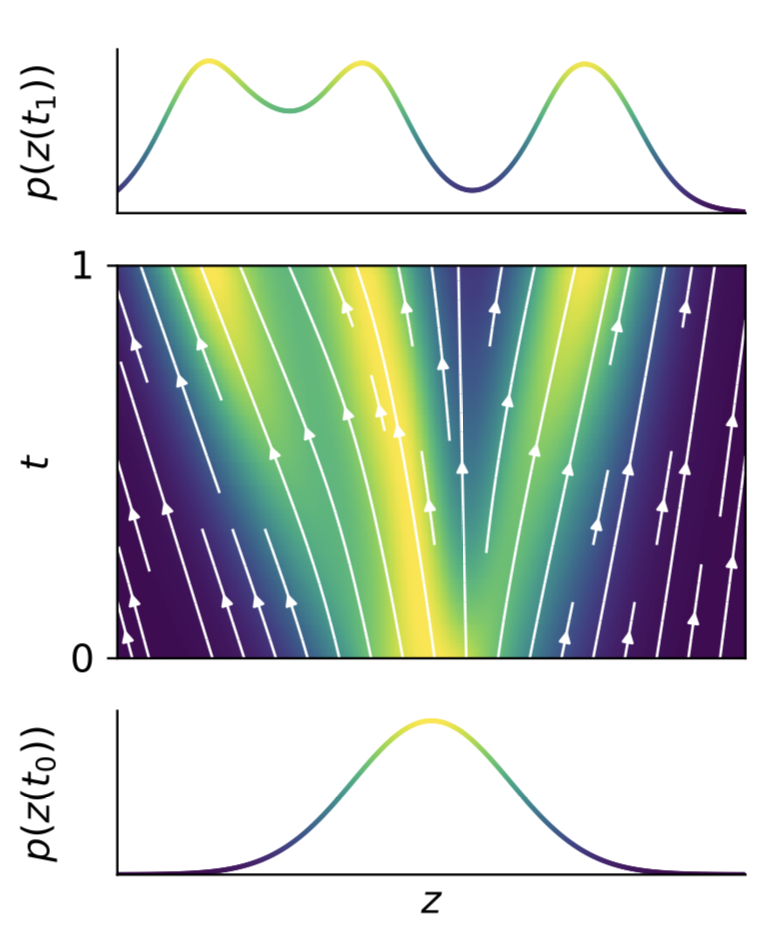
\includegraphics[width=0.75\linewidth]{figs/cnf_flow.png}
		\end{figure}
	\end{minipage}%
	\begin{minipage}[t]{0.6\columnwidth}
		\begin{figure}
			  \centering
			  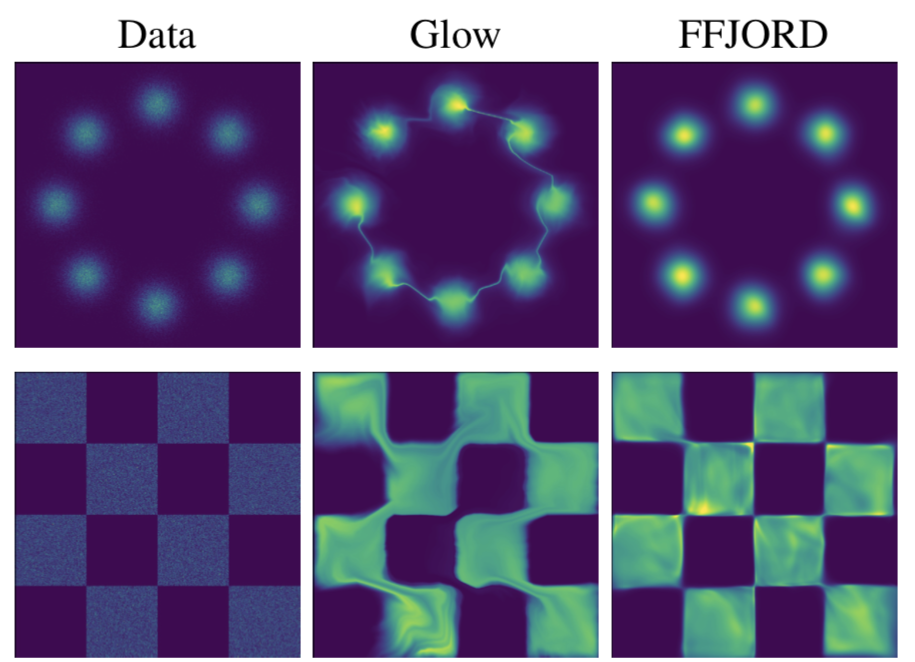
\includegraphics[width=0.8\linewidth]{figs/ffjord.png}
		\end{figure}
	\end{minipage}
	\myfootnotewithlink{https://arxiv.org/abs/1810.01367}{Grathwohl W. et al. FFJORD: Free-form Continuous Dynamics for Scalable Reversible Generative Models, 2018} 
\end{frame}
%=======
\begin{frame}{Continuous Normalizing Flows}
	\vspace{0.2cm}
	\begin{itemize}
		\item $\text{tr} \left( \frac{\partial f(\bz(t), \btheta)}{\partial \bz(t)} \right)$ costs $O(m^2)$ ($m$
		evaluations of $f$), since we have to compute a derivative for each diagonal element. 
		\item Vector-Jacobian products ${\color{violet}\bv^T \frac{\partial f}{\partial \bz}}$ can be computed for approximately the same cost as evaluating $f$.
	\end{itemize}
	It is possible to reduce cost from $O(m^2)$ to $O(m)$!
	\begin{block}{Hutchinson's trace estimator}
		\vspace{-0.3cm}
		\[
		    \text{tr}(A) = \text{tr}\left(A\mathbb{E}_{p(\bepsilon)} \left[ \bepsilon \bepsilon^T \right]\right) = \mathbb{E}_{p(\bepsilon)} \left[ {\color{violet} \bepsilon^T A} \bepsilon  \right]; \quad \mathbb{E} [\bepsilon] = 0; \quad \text{Cov} (\bepsilon) = I.
		\]
		\vspace{-0.5cm}
	\end{block}
	\begin{block}{FFJORD density estimation}
		\vspace{-0.8cm}
		\begin{multline*}
		    \log p(\bz(t_1)) = \log p(\bz(t_0)) - \int_{t_0}^{t_1} \text{tr}  \left( \frac{\partial f (\bz(t), \btheta)}{\partial \bz(t)} \right) dt = \\ = \log p(\bz(t_0)) - \mathbb{E}_{p(\bepsilon)} \int_{t_0}^{t_1} \left[ {\color{violet}\bepsilon^T \frac{\partial f}{\partial \bz}} \bepsilon \right] dt.
		\end{multline*}
	\end{block}
	\myfootnotewithlink{https://arxiv.org/abs/1810.01367}{Grathwohl W. et al. FFJORD: Free-form Continuous Dynamics for Scalable Reversible Generative Models, 2018} 
\end{frame}
%=======
\section{Langevin dynamic}
%=======
\begin{frame}{Generative models zoo}
	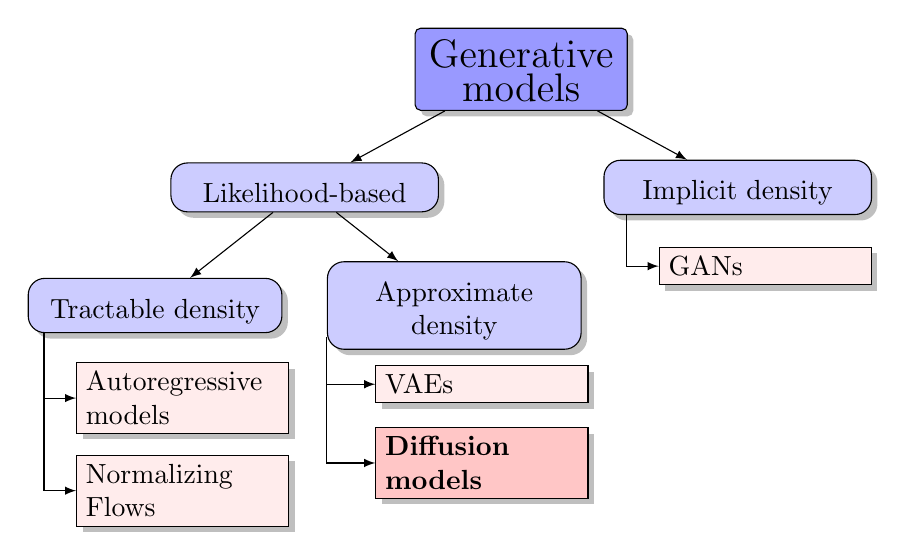
\begin{tikzpicture}[
	 	basic/.style  = {draw, text width=2cm, drop shadow, rectangle},
	 	root/.style   = {basic, rounded corners=2pt, thin, text height=1.1em, text width=7em, align=center, fill=blue!40},
	 	level 1/.style={sibling distance=55mm},
	 	level 2/.style = {basic, rounded corners=6pt, thin, align=center, fill=blue!20, text height=1.1em, text width=9em, sibling distance=38mm},
	 	level 3/.style = {basic, rounded corners=6pt, thin,align=center, fill=blue!20, text width=8.5em},
	 	level 4/.style = {basic, thin, align=left, fill=pink!30, text width=7em},
	 	level 5/.style = {basic, thin, align=left, fill=pink!90, text width=7em},
		edge from parent/.style={->,draw},
		>=latex]
		
		% root of the the initial tree, level 1
		\node[root] {\Large Generative models}
		% The first level, as children of the initial tree
		child {node[level 2] (c1) {Likelihood-based}
			child {node[level 3] (c11) {Tractable density}}
			child {node[level 3] (c12) {Approximate density}}
		}
		child {node[level 2] (c2) {Implicit density}};
	
		% The second level, relatively positioned nodes
		\begin{scope}[every node/.style={level 4}]
			\node [below of = c11, yshift=-5pt, xshift=10pt] (c111) {Autoregressive models};
			\node [below of = c111, yshift=-5pt] (c112) {Normalizing Flows};
			\node [below of = c12, xshift=10pt] (c121) {VAEs};
			
			\node [below of = c2, xshift=10pt] (c21) {GANs};
		\end{scope}
				
		% The second level, relatively positioned nodes
		\begin{scope}[every node/.style={level 5}]
			\node [below of = c121] (c122) {\textbf{Diffusion \\ models}};
		\end{scope}
	
		% lines from each level 1 node to every one of its "children"
		\foreach \value in {1,2}
		\draw[->] (c11.194) |- (c11\value.west);
		
		\foreach \value in {1,2}
		\draw[->] (c12.194) |- (c12\value.west);
		
		\draw[->] (c2.194) |- (c21.west);
		
	\end{tikzpicture}
\end{frame}
%=======
\begin{frame}{Langevin dynamic}
	Imagine that we have some generative model $p(\bx | \btheta)$.
	\begin{block}{Statement}
		Let $\bx_0$ be a random vector. Then under mild regularity conditions for small enough $\eta$ samples from the following dynamics
		\[
			\bx_{t + 1} = \bx_t + \eta \frac{1}{2} \nabla_{\bx_t} \log p(\bx_t | \btheta) + \sqrt{\eta} \cdot \bepsilon, \quad \bepsilon \sim \cN(0, 1).
		\]
		will comes from $p(\bx | \btheta)$.
	\end{block}
	What do we get if $\bepsilon = \boldsymbol{0}$?
	\begin{block}{Energy-based model}
		\[
			p(\bx | \btheta) = \frac{\hat{p}(\bx | \btheta)}{Z_{\btheta}}, \quad \text{where } Z_{\theta} = \int \hat{p}(\bx | \btheta) d \bx
		\]
		\[
			\nabla_{\bx} \log p(\bx | \btheta) = \nabla_{\bx} \log \hat{p}(\bx | \btheta) - \nabla_{\bx} \log Z_{\btheta} = \nabla_{\bx} \log \hat{p}(\bx | \btheta)
		\]
	\end{block}
\end{frame}
%=======
\begin{frame}{Stochastic differential equation (SDE)}
	Let define stochastic process $\bx(t)$ with initial condition $bx(0) \sim p_0(\bx)$:
	\[
		d\bx = \mathbf{f}(\bx, t) dt + g(t) d \bw
	\]
	\vspace{-0.6cm}
	\begin{itemize}
		\item $\bw(t)$ is the standard Wiener process (Brownian motion)
		\[		
			\bw(t) - \bw(s) \sim \cN(0, t - s), \quad d \bw = \epsilon \cdot \sqrt{dt}, \, \text{where } \epsilon \sim \cN(0, 1).
		\]
		 \item $\mathbf{f}(\bx, t)$ is the \textbf{drift} function of $\bx(t)$.
		 \item $g(t)$ is the \textbf{diffusion} coefficient of $\bx(t)$.
		 \item If $g(t) = 0$ we get standard ODE.
	\end{itemize}
	 How to get distribution $p(\bx, t)$ for $\bx(t)$?
 	\begin{block}{Theorem (Kolmogorov-Fokker-Planck)}
 		Evolution of the distribution $p(\bx | t)$ is given by the folliwing ODE:
 		\vspace{-0.2cm}
 		\[
 			\frac{\partial p(\bx, t)}{\partial t} = \text{tr}\left(- \frac{\partial}{\partial \bx} \bigl[ \mathbf{f}(\bx, t) p(\bx, t)\bigr] + \frac{1}{2} g^2(t) \frac{\partial^2 p(\bx, t)}{\partial \bx^2} \right)
 		\]
 		\vspace{-0.6cm}
 	\end{block}
\end{frame}
%=======
\begin{frame}{Stochastic differential equation (SDE)}
	\[
		d\bx = {\color{violet}\mathbf{f}(\bx, t)} dt + {\color{cyan}g(t)} d \bw
	\]
	\vspace{-0.4cm}
	\begin{block}{Langevin SDE (special case)}
		\vspace{-0.3cm}
		\[
			d \bx = {\color{violet}\frac{1}{2} \frac{\partial}{\partial \bx} \log p(\bx, t)} d t + {\color{cyan} 1 }d \bw
		\]
		\vspace{-0.6cm}
	\end{block}
	\begin{block}{Langevin discrete dynamic}
		\vspace{-0.3cm}
		\[
			\bx_{t + 1} = \bx_t + \eta \frac{1}{2} \frac{\partial}{\partial \bx} \log p(\bx, t) + \sqrt{\eta} \cdot \bepsilon, \quad \bepsilon \sim \cN(0, 1).
		\]
		\vspace{-0.3cm}
	\end{block}
	Let apply KFP theorem.
	\begin{multline*}
		\frac{\partial p(\bx, t)}{\partial t} =  \text{tr} \left(- \frac{\partial}{\partial \bx}\left[ p(\bx, t) \frac{1}{2} \frac{\partial}{\partial \bx} \log p(\bx, t) \right]  + \frac{1}{2} \frac{\partial^2 p(\bx, t)}{\partial \bx^2} \right) = \\
		= \text{tr} \left(- \frac{\partial}{\partial \bx}\left[ \frac{1}{2} \frac{\partial}{\partial \bx} p(\bx, t) \right]  + \frac{1}{2} \frac{\partial^2 p(\bx, t)}{\partial \bx^2} \right) = 0
	\end{multline*}
	The density $p(\bx, t) = \text{const}$.
\end{frame}
%=======
\begin{frame}{Stochastic differential equation (SDE)}
	\begin{block}{Statement}
		Let $\bx_0$ be a random vector. Then samples from the following dynamics
		\[
			\bx_{t + 1} = \bx_t + \eta \frac{1}{2} \nabla_{\bx_t} \log p(\bx_t | \btheta) + \sqrt{\eta} \cdot \bepsilon, \quad \bepsilon \sim \cN(0, 1).
		\]
		will come from $p(\bx | \btheta)$ under mild regularity conditions for small enough $\eta$ and large enough $t$.
	\end{block}
	\begin{minipage}{0.6\linewidth}
		The density $p(\bx | \btheta)$ is a \textbf{stationary} distribution for this SDE.
	\end{minipage}%
	\begin{minipage}{0.35\linewidth}
		\vspace{-0.2cm}
		\begin{figure}
			\centering
			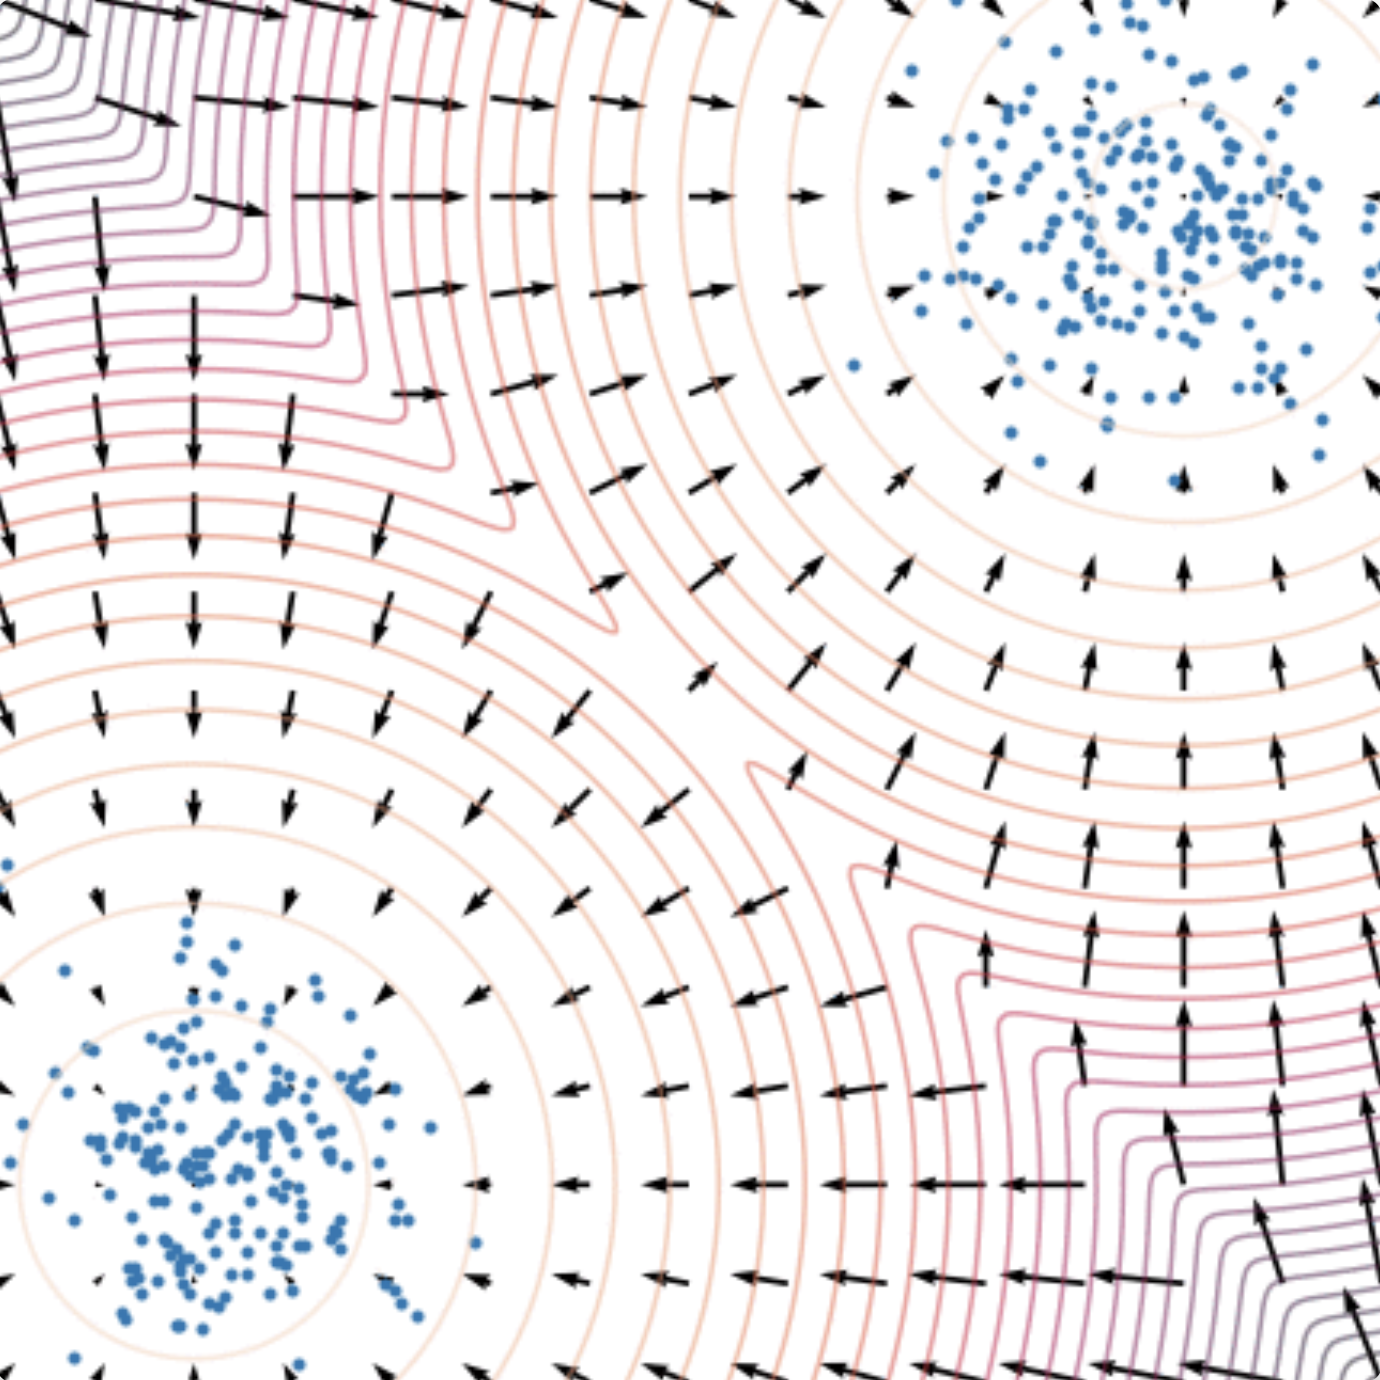
\includegraphics[width=0.9\linewidth]{figs/langevin_dynamic}
		\end{figure}
	\end{minipage}
	\myfootnotewithlink{https://yang-song.github.io/blog/2019/ssm/}{Song Y. Generative Modeling by Estimating Gradients of the Data Distribution, blog post, 2021} 
	\end{frame}
%=======
\section{Score matching}
%=======
\begin{frame}{Score matching}
	We could sample from the model if we have $\nabla_{\bx}\log p(\bx| \btheta)$.
	\begin{block}{Fisher divergence}
		\vspace{-0.3cm}
		\[
			D_F(\pi, p) = \frac{1}{2}\bbE_{\pi}\bigl\| \nabla_{\bx}\log p(\bx| \btheta) - \nabla_\bx \log \pi(\bx) \bigr\|^2_2 \rightarrow \min_{\btheta}
		\]
		\vspace{-0.5cm}
	\end{block}
	\begin{block}{Score function}
		\vspace{-0.3cm}
		\[
			\bs(\bx, \btheta) = \nabla_{\bx}\log p(\bx| \btheta)
		\]
	\end{block}
	\textbf{Problem:} we do not know $\nabla_\bx \log \pi(\bx)$.
	\begin{block}{Theorem}
		\vspace{-0.6cm}
		\[
			\frac{1}{2} \bbE_{\pi}\bigl\| \bs(\bx, \btheta) - \nabla_\bx \log \pi(\bx) \bigr\|^2_2 = \bbE_{\pi}\Bigr[ \frac{1}{2}\| \bs(\bx, \btheta) \|_2^2 + \text{tr}\bigl(\nabla_{\bx} \bs(\bx, \btheta)\bigr) \Bigr] + \text{const}
		\]
		\vspace{-0.4cm}
	\end{block}
	Here $\nabla_{\bx} \bs(\bx, \btheta) = \nabla_{\bx}^2 \log p(\bx | \btheta)$ is a Hessian matrix.
	\myfootnotewithlink{https://jmlr.org/papers/volume6/hyvarinen05a/old.pdf}{Hyvarinen A. Estimation of non-normalized statistical models by score matching, 2005} 
\end{frame}
%=======
\begin{frame}{Score matching}
	\begin{block}{Theorem}
		\vspace{-0.6cm}
		\[
			\frac{1}{2} \bbE_{\pi}\bigl\| \bs(\bx, \btheta) - \nabla_\bx \log \pi(\bx) \bigr\|^2_2 = \bbE_{\pi}\Bigr[ \frac{1}{2}\| \bs(\bx, \btheta) \|_2^2 + \text{tr}\bigl(\nabla_{\bx} \bs(\bx, \btheta)\bigr) \Bigr] + \text{const}
		\]
		\vspace{-0.6cm}
	\end{block}
	\begin{block}{Proof (only for 1D)}
		\vspace{-0.6cm}
		{\small
		\begin{multline*}
			\bbE_{\pi}\bigl\| s(x) - \nabla_x \log \pi(x) \bigr\|^2_2 = \bbE_{\pi} \bigl[ s(x)^2 + (\nabla_x \log \pi(x))^2 - 2{\color{teal}[s(x) \nabla_x \log \pi(x) ] \bigr] }
		\end{multline*}
		\vspace{-0.8cm}
		\begin{align*}
			{\color{teal}\bbE_{\pi} [{\color{violet}s(x) } \nabla_x \log \pi(x) ] } &= \int {\color{olive}\pi(x) {\color{violet}\nabla_x \log p(x)} \nabla_x \log \pi(x)} d x \\ 
			&= \int {\color{violet}\nabla_x \log p(x) } {\color{olive}\nabla_x \pi(x) } dx = \Bigl.\pi(x) \nabla_x \log p(x) \Bigr|_{-\infty}^{+\infty} \\
			&- \int \nabla^2_x \log p(x)  \pi(x) dx =- \bbE_{\pi} \nabla^2_x \log p(x)
		\end{align*}
		\[
			\frac{1}{2} \bbE_{\pi}\bigl\| s(x) - \nabla_x \log \pi(x) \bigr\|^2_2 = \frac{1}{2} \bbE_{\pi} \Bigr[s(x)^2 + \nabla_x s(x) \Bigl]+ \text{const}.
		\]
		}
	\end{block}
	\myfootnotewithlink{https://jmlr.org/papers/volume6/hyvarinen05a/old.pdf}{Hyvarinen A. Estimation of non-normalized statistical models by score matching, 2005} 
\end{frame}
%=======
\begin{frame}{Score matching}
	\vspace{-0.3cm}
	\begin{figure}
		\centering
		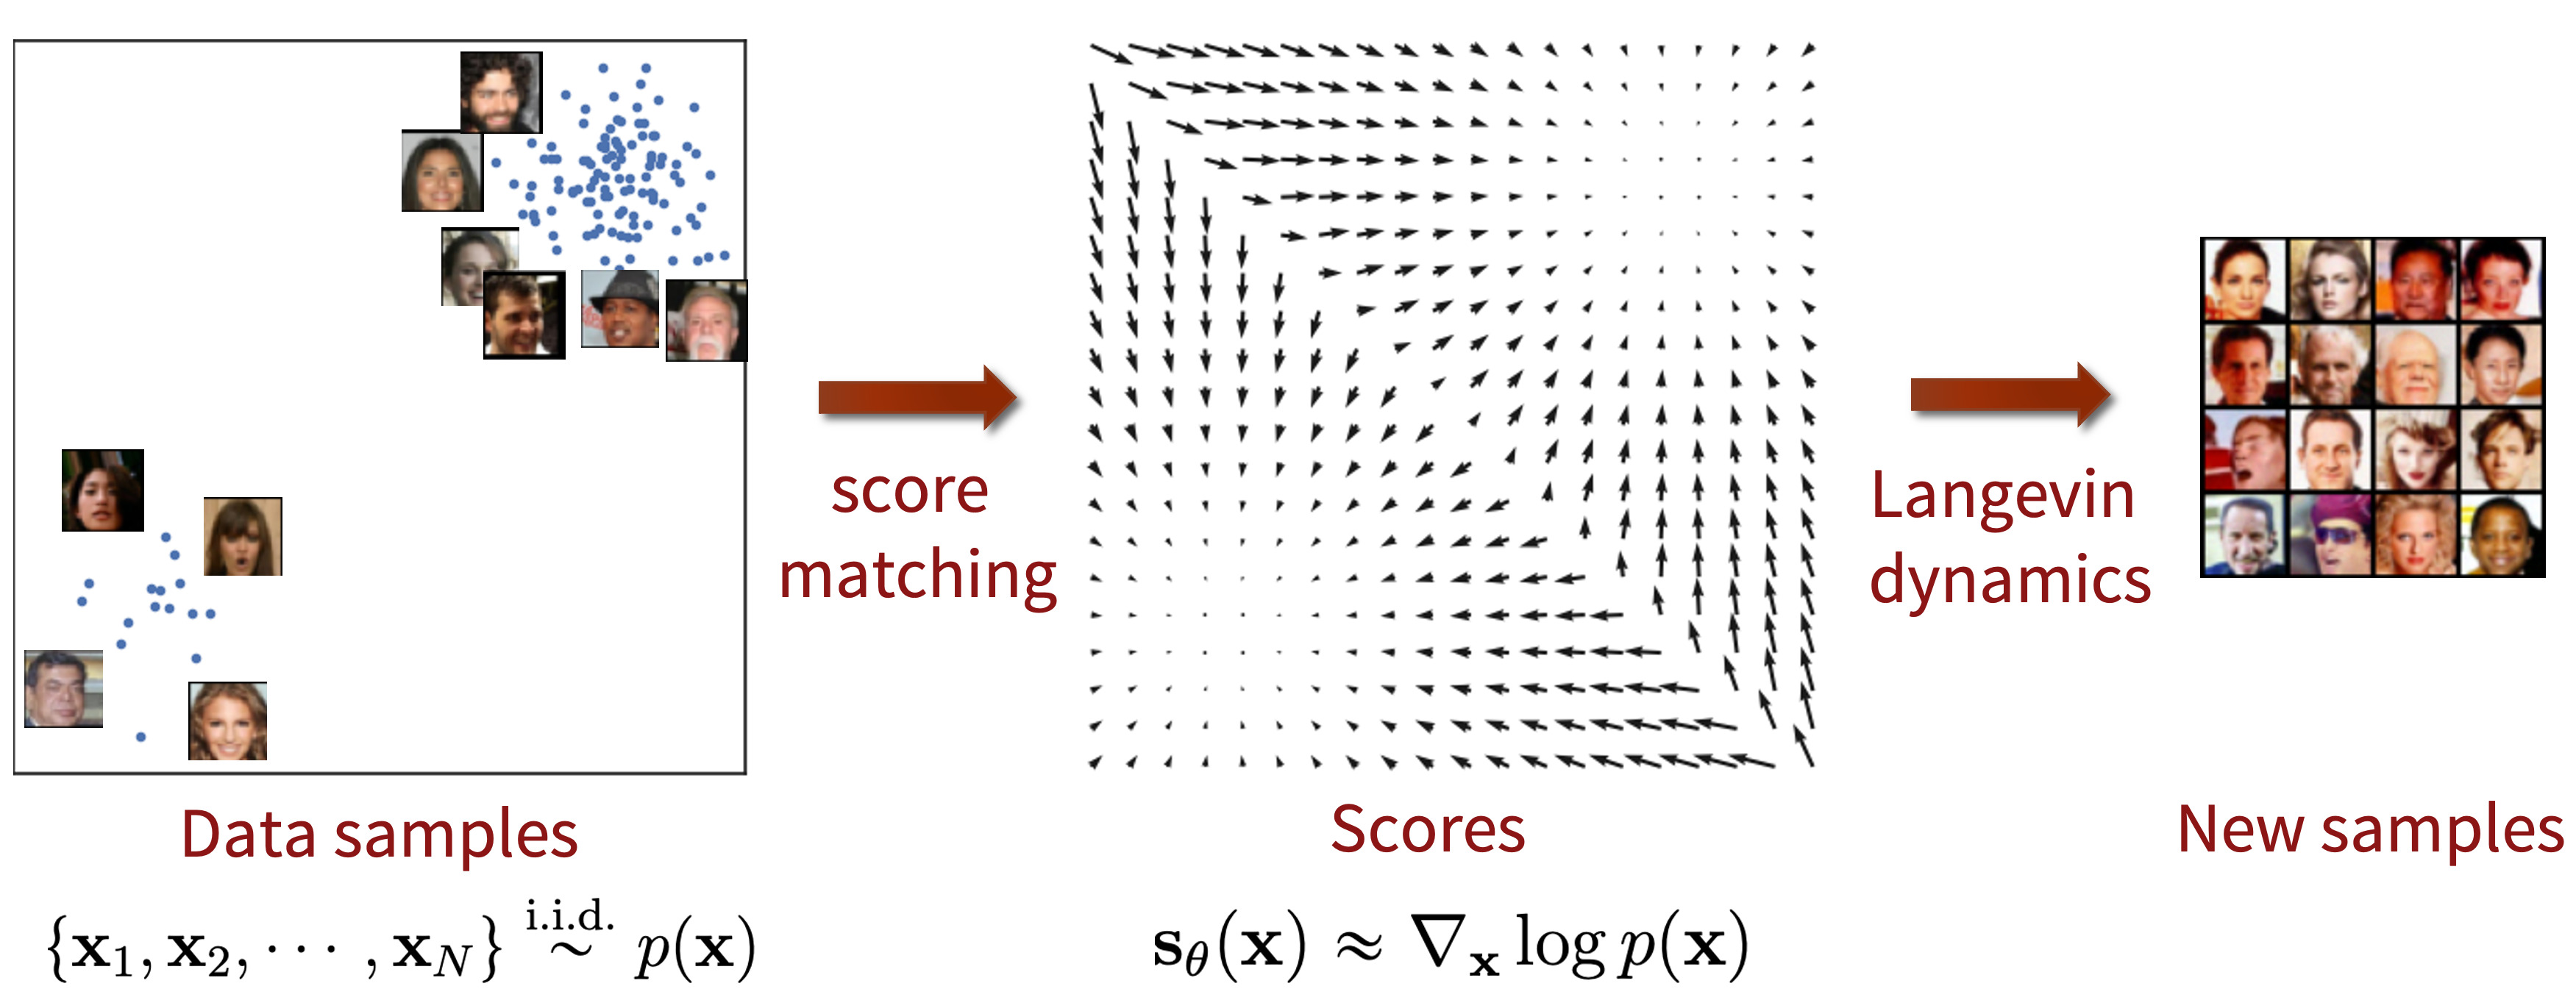
\includegraphics[width=0.8\linewidth]{figs/smld}
	\end{figure}
	\vspace{-0.6cm}
	\begin{block}{Theorem}
		\vspace{-0.6cm}
		\[
			\frac{1}{2} \bbE_{\pi}\bigl\| \bs(\bx, \btheta) - \nabla_\bx \log \pi(\bx) \bigr\|^2_2 = \bbE_{\pi}\Bigr[ \frac{1}{2}\| \bs(\bx, \btheta) \|_2^2 + \text{tr}\bigl(\nabla_{\bx} \bs(\bx, \btheta)\bigr) \Bigr] + \text{const}
		\]
		\vspace{-0.4cm}
	\end{block}
	\begin{enumerate}
	    \item The left hand side is intractable due to unknown $\pi(\bx)$ -- \textbf{denoising score matching}. 
	    \item The right hand side is complex due to Hessian matrix -- \textbf{sliced score matching}.
	\end{enumerate}
	\myfootnotewithlink{https://yang-song.github.io/blog/2019/ssm/}{Song Y. Generative Modeling by Estimating Gradients of the Data Distribution, blog post, 2021}
\end{frame}
%=======
\begin{frame}{Score matching}
	\begin{block}{Sliced score matching (Hutchinson's trace estimation)}
		\vspace{-0.3cm}
		\[
			\bbE_{\pi}\Bigr[ \text{tr}\bigl(\nabla_{\bx} \bs(\bx, \btheta)\bigr) \Bigr] = \bbE_{\pi(\bx)} \mathbb{E}_{p(\bepsilon)} \left[ {\color{violet}\bepsilon^T \nabla_{\bx} \bs(\bx, \btheta)} \bepsilon \right],
		\]
		where $\mathbb{E} [\bepsilon] = 0$ and $\text{Cov} (\bepsilon) = I$.
	\end{block}
	\begin{block}{Denoising score mathing}
		Let perturb original data by normal noise $p(\bx | \bx', \sigma) = \cN(\bx | \bx', \sigma^2 \bI)$
		\vspace{-0.3cm}
		\[
			\pi(\bx | \sigma) = \int \pi(\bx') p(\bx | \bx', \sigma) d\bx'.
		\]
		\vspace{-0.6cm} \\
		Then the solution of 
		\[
			\frac{1}{2} \bbE_{\pi(\bx | \sigma)}\bigl\| \bs(\bx, \btheta, \sigma) - \nabla_\bx \log \pi(\bx | \sigma) \bigr\|^2_2 \rightarrow \min_{\btheta}
		\]
		satisfies $\bs(\bx, \btheta, \sigma) = \bs(\bx, \btheta, 0) = \bs(\bx, \btheta)$ using small enough noise scale $\sigma$.
	\end{block}
	\myfootnotewithlink{https://arxiv.org/abs/1905.07088}{Song Y. Sliced Score Matching: A Scalable Approach to Density and Score Estimation, 2019}
\end{frame}
%=======
\begin{frame}{Denoising score matching}
	\begin{block}{Theorem}
		\vspace{-0.8cm}
		\begin{multline*}
			\bbE_{\pi(\bx | \sigma)}\bigl\| \bs(\bx, \btheta, \sigma) - \nabla_\bx \log \pi(\bx | \sigma) \bigr\|^2_2 = \\ = \bbE_{\pi(\bx')} \bbE_{p(\bx | \bx', \sigma)}\bigl\| \bs(\bx, \btheta, \sigma) - \nabla_\bx \log p(\bx | \bx', \sigma) \bigr\|^2_2	
		\end{multline*}
		\vspace{-0.8cm}
	\end{block}
	\begin{figure}
		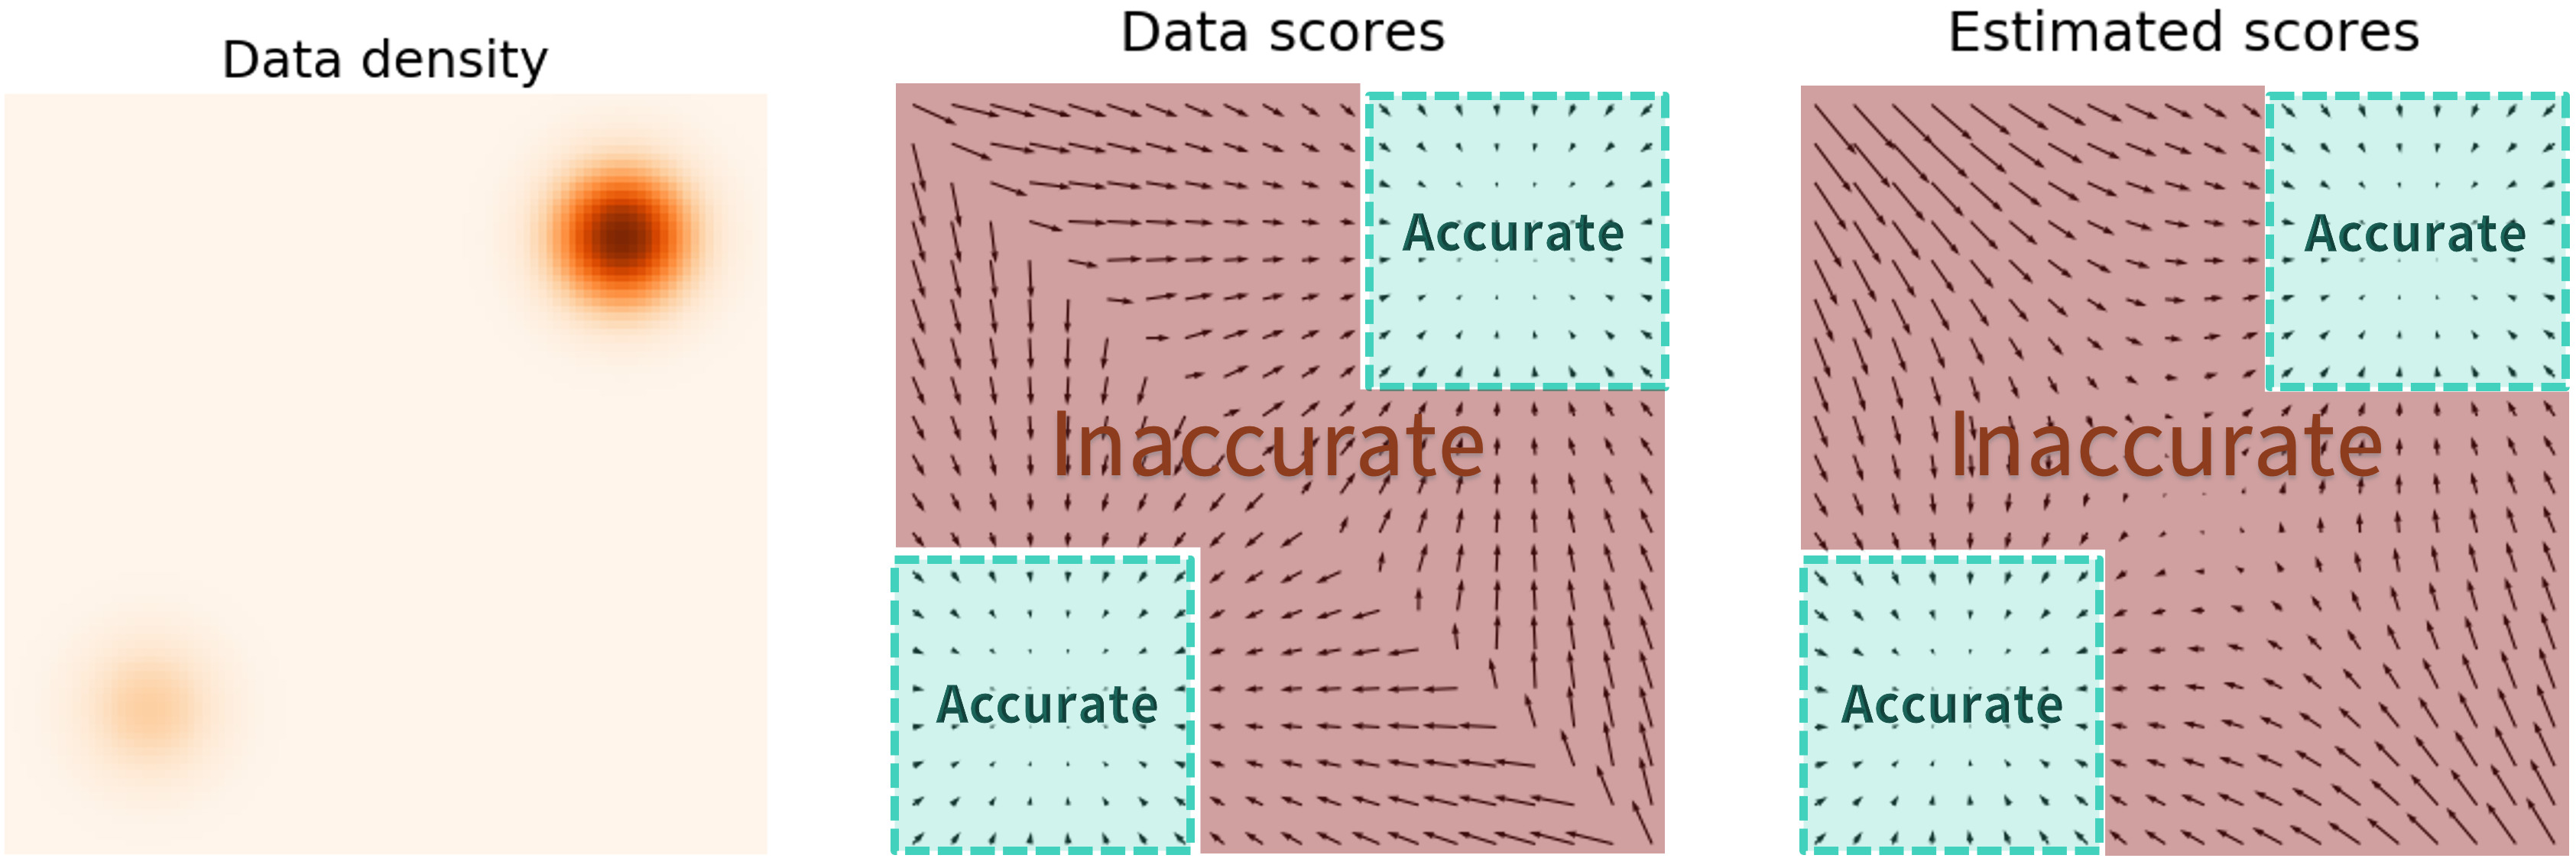
\includegraphics[width=0.75\linewidth]{figs/pitfalls}
		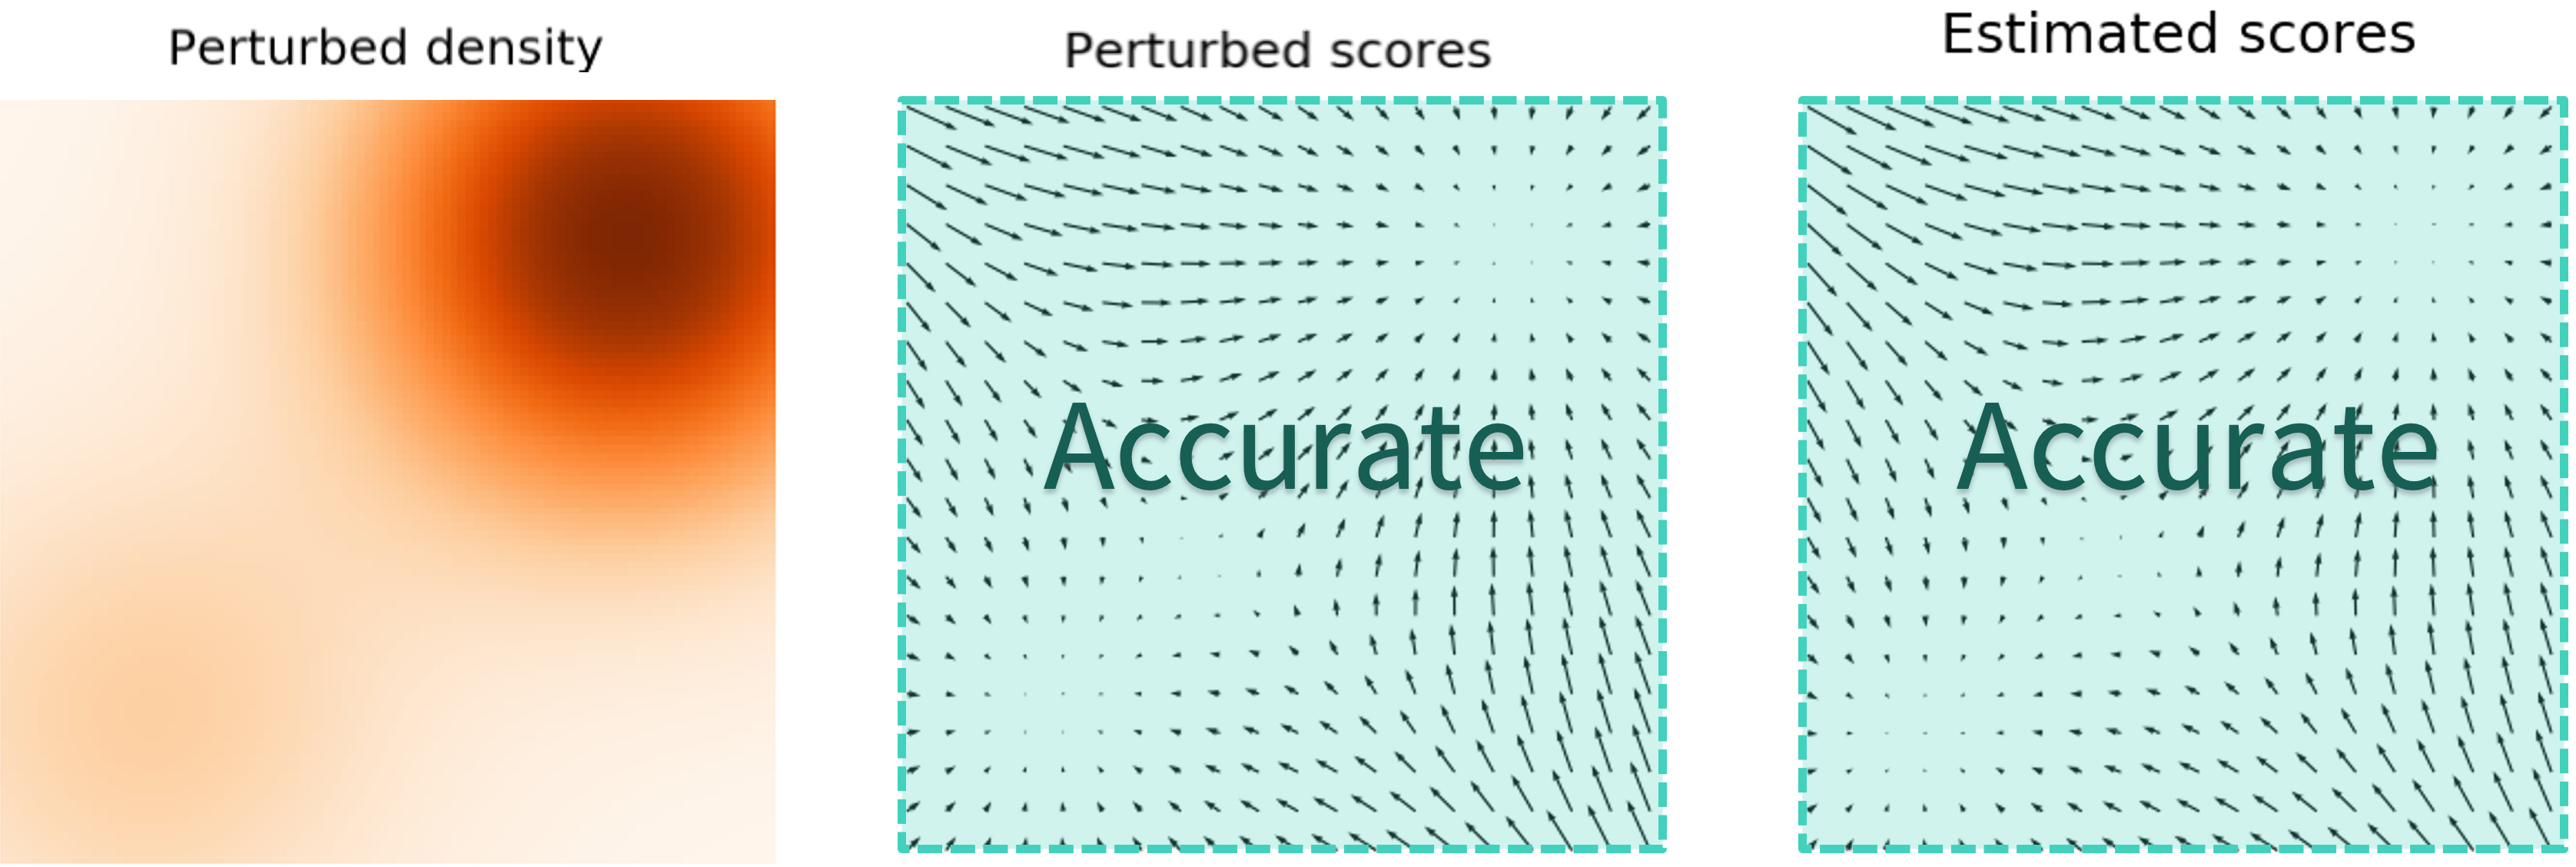
\includegraphics[width=0.75\linewidth]{figs/single_noise}
	\end{figure}
	\myfootnotewithlink{https://yang-song.github.io/blog/2019/ssm/}{Song Y. Generative Modeling by Estimating Gradients of the Data Distribution, blog post, 2021}
\end{frame}
%=======
\begin{frame}{Summary}
	\begin{itemize}
		\item Adjoint method generalizes backpropagation procedure and allows to train Neural ODE solving ODE for adjoint function back in time.
		\vfill
		\item Kolmogorov-Fokker-Planck theorem allows to construct continuous-in-time normalizing flow with less functional restrictions.
		\vfill
		\item FFJORD model makes such kind of flows scalable.
		\vfill
	\end{itemize}
\end{frame}
\end{document} 